\appendix % Anhang

    % Kapiteln mit Buchstaben beziffern
    %\renewcommand*\thechapter{\Alph{chapter}}
    \renewcommand{\thetable}{\Alph{table}}
    \setcounter{table}{0}
    \renewcommand{\thefigure}{\Alph{figure}}
    \setcounter{figure}{0}

\section{Anhang}
\subsection{Abbildungen}

\begin{figure}[h]
    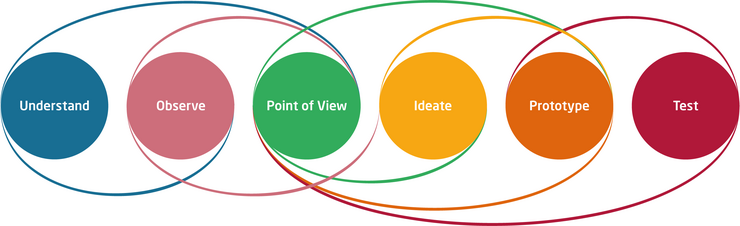
\includegraphics[width=\textwidth]{img/DT_process.png}
    \caption{The Design Thinking Process \#todo ref}
    \label{fig:dt_process}
\end{figure} 

\begin{figure}[h]
    \begin{center}
        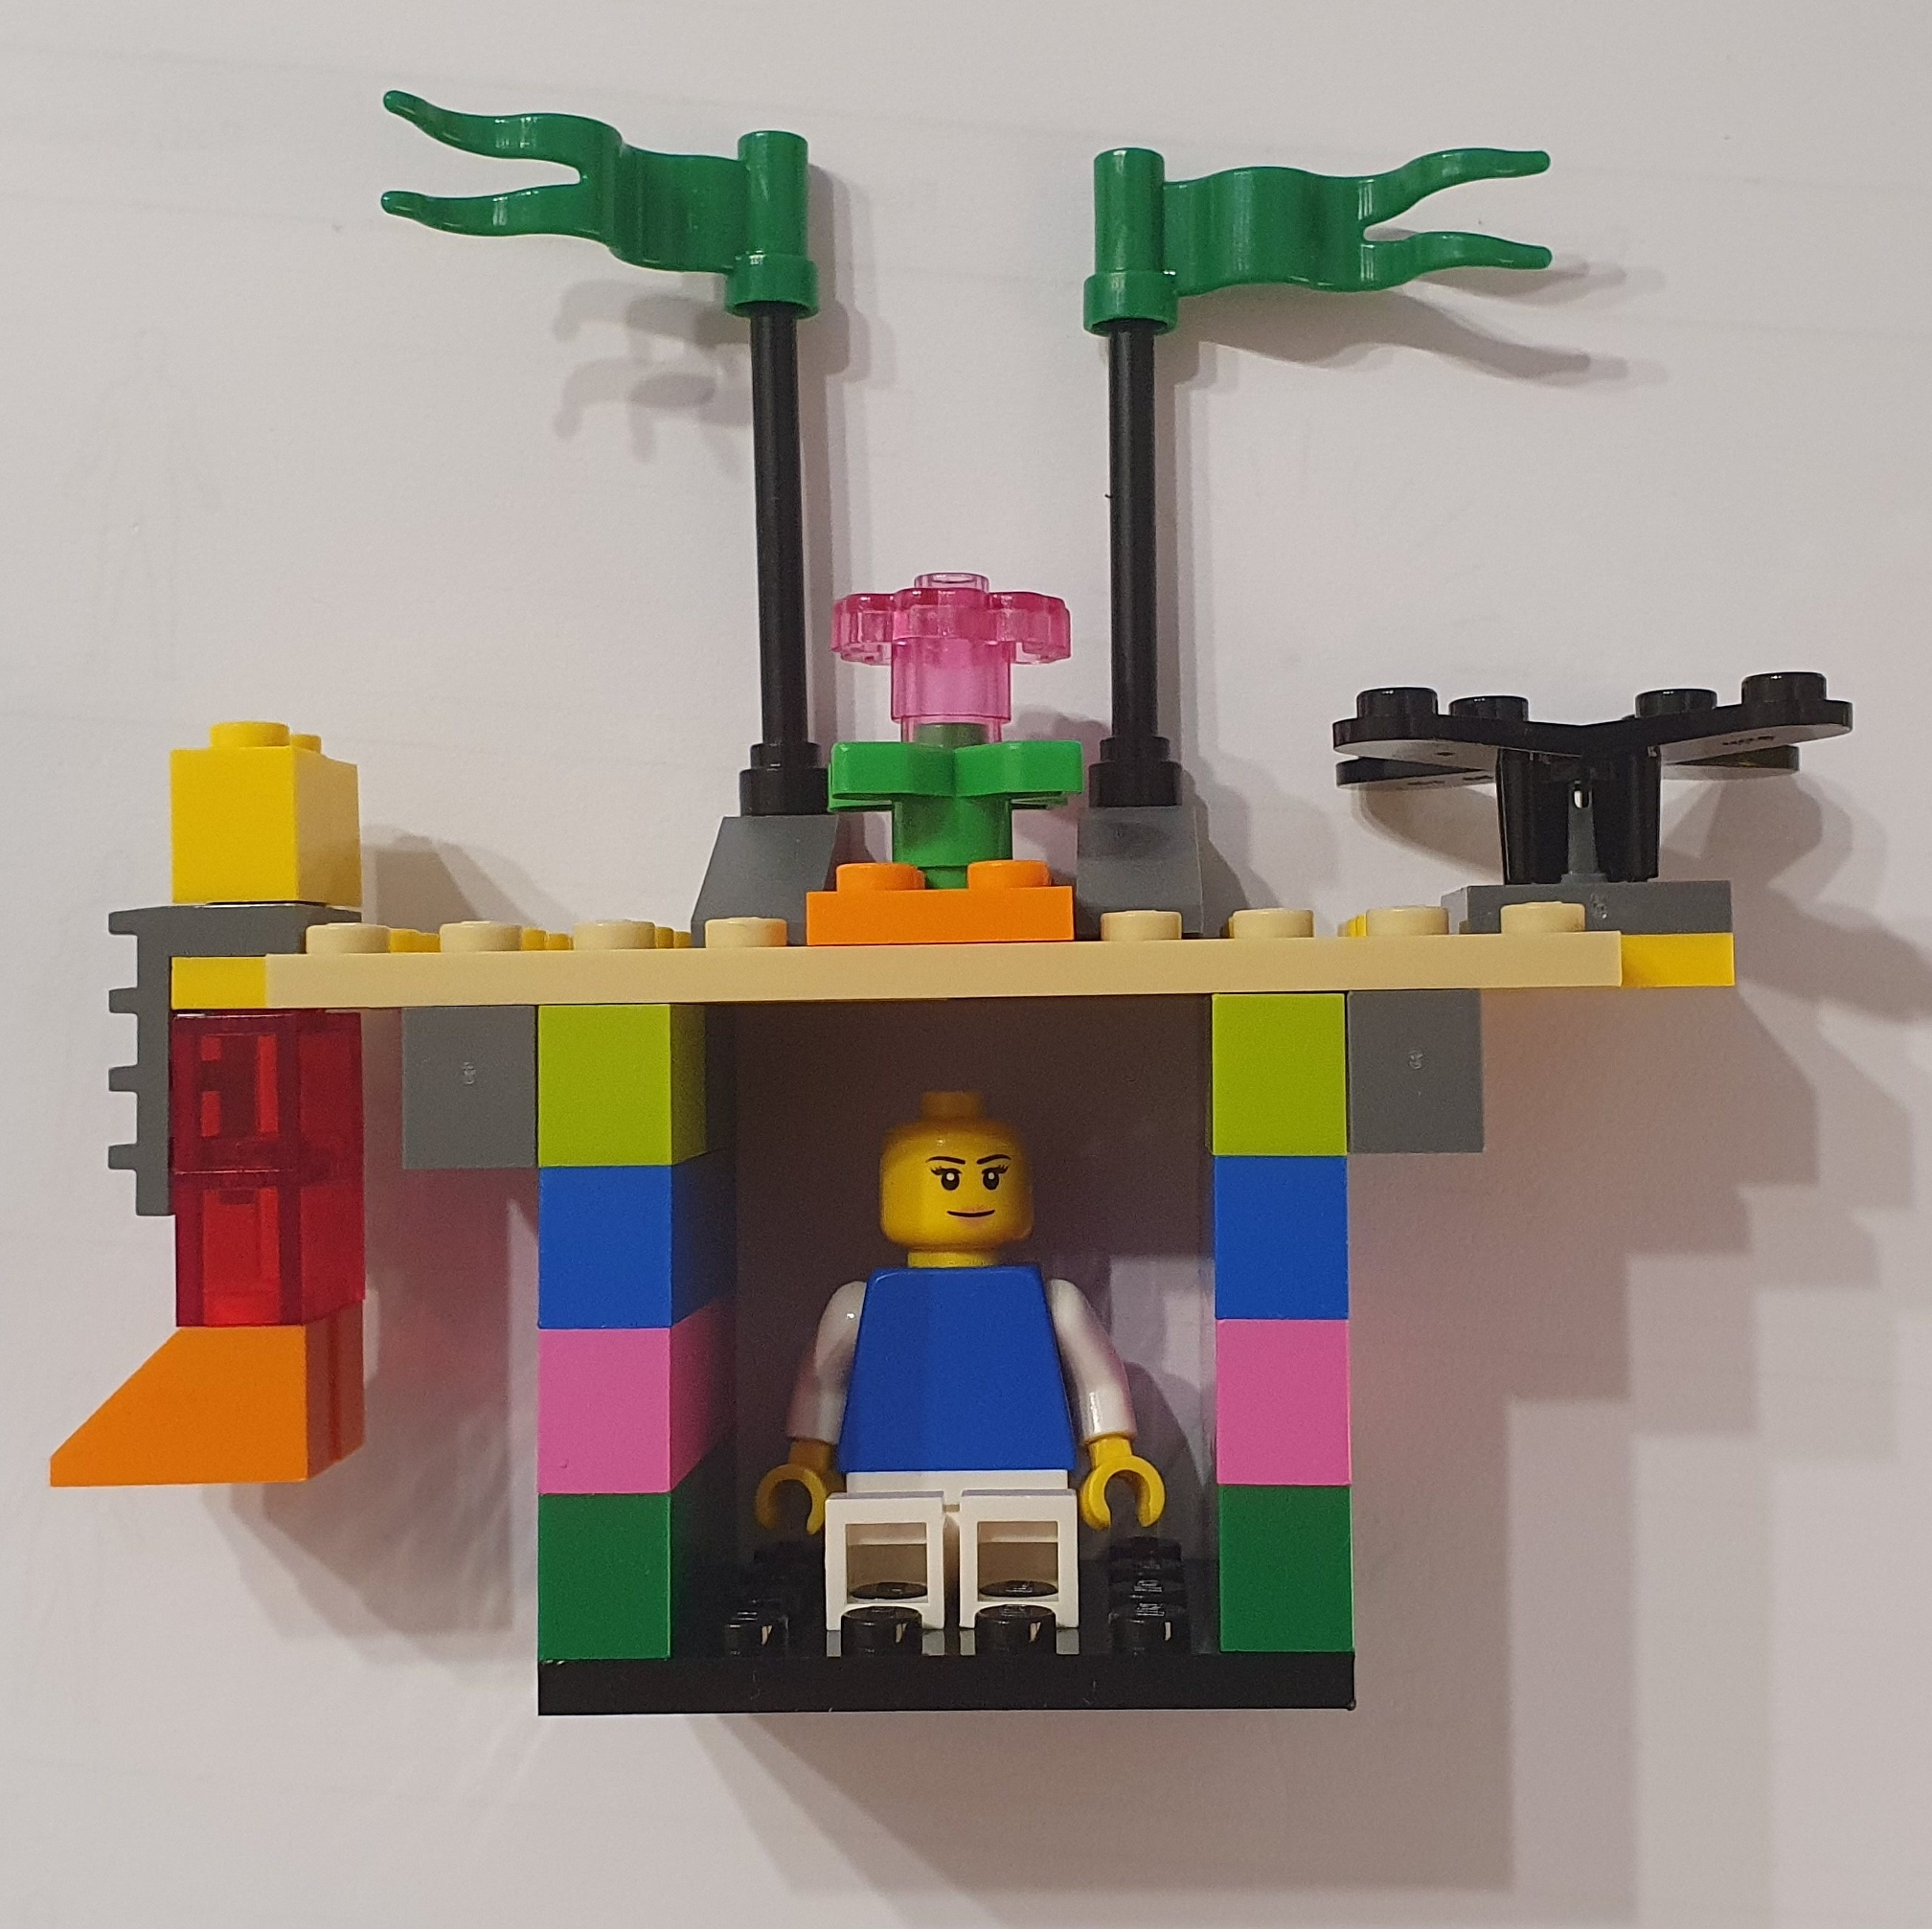
\includegraphics[width=7.5cm]{img/week_2.jpg}
    \end{center}
    \caption{``My 2020'' - Prototype of week 2}
    \label{fig:week2}
\end{figure} 
\begin{center}
    \begin{figure}[h]
        \begin{center}
            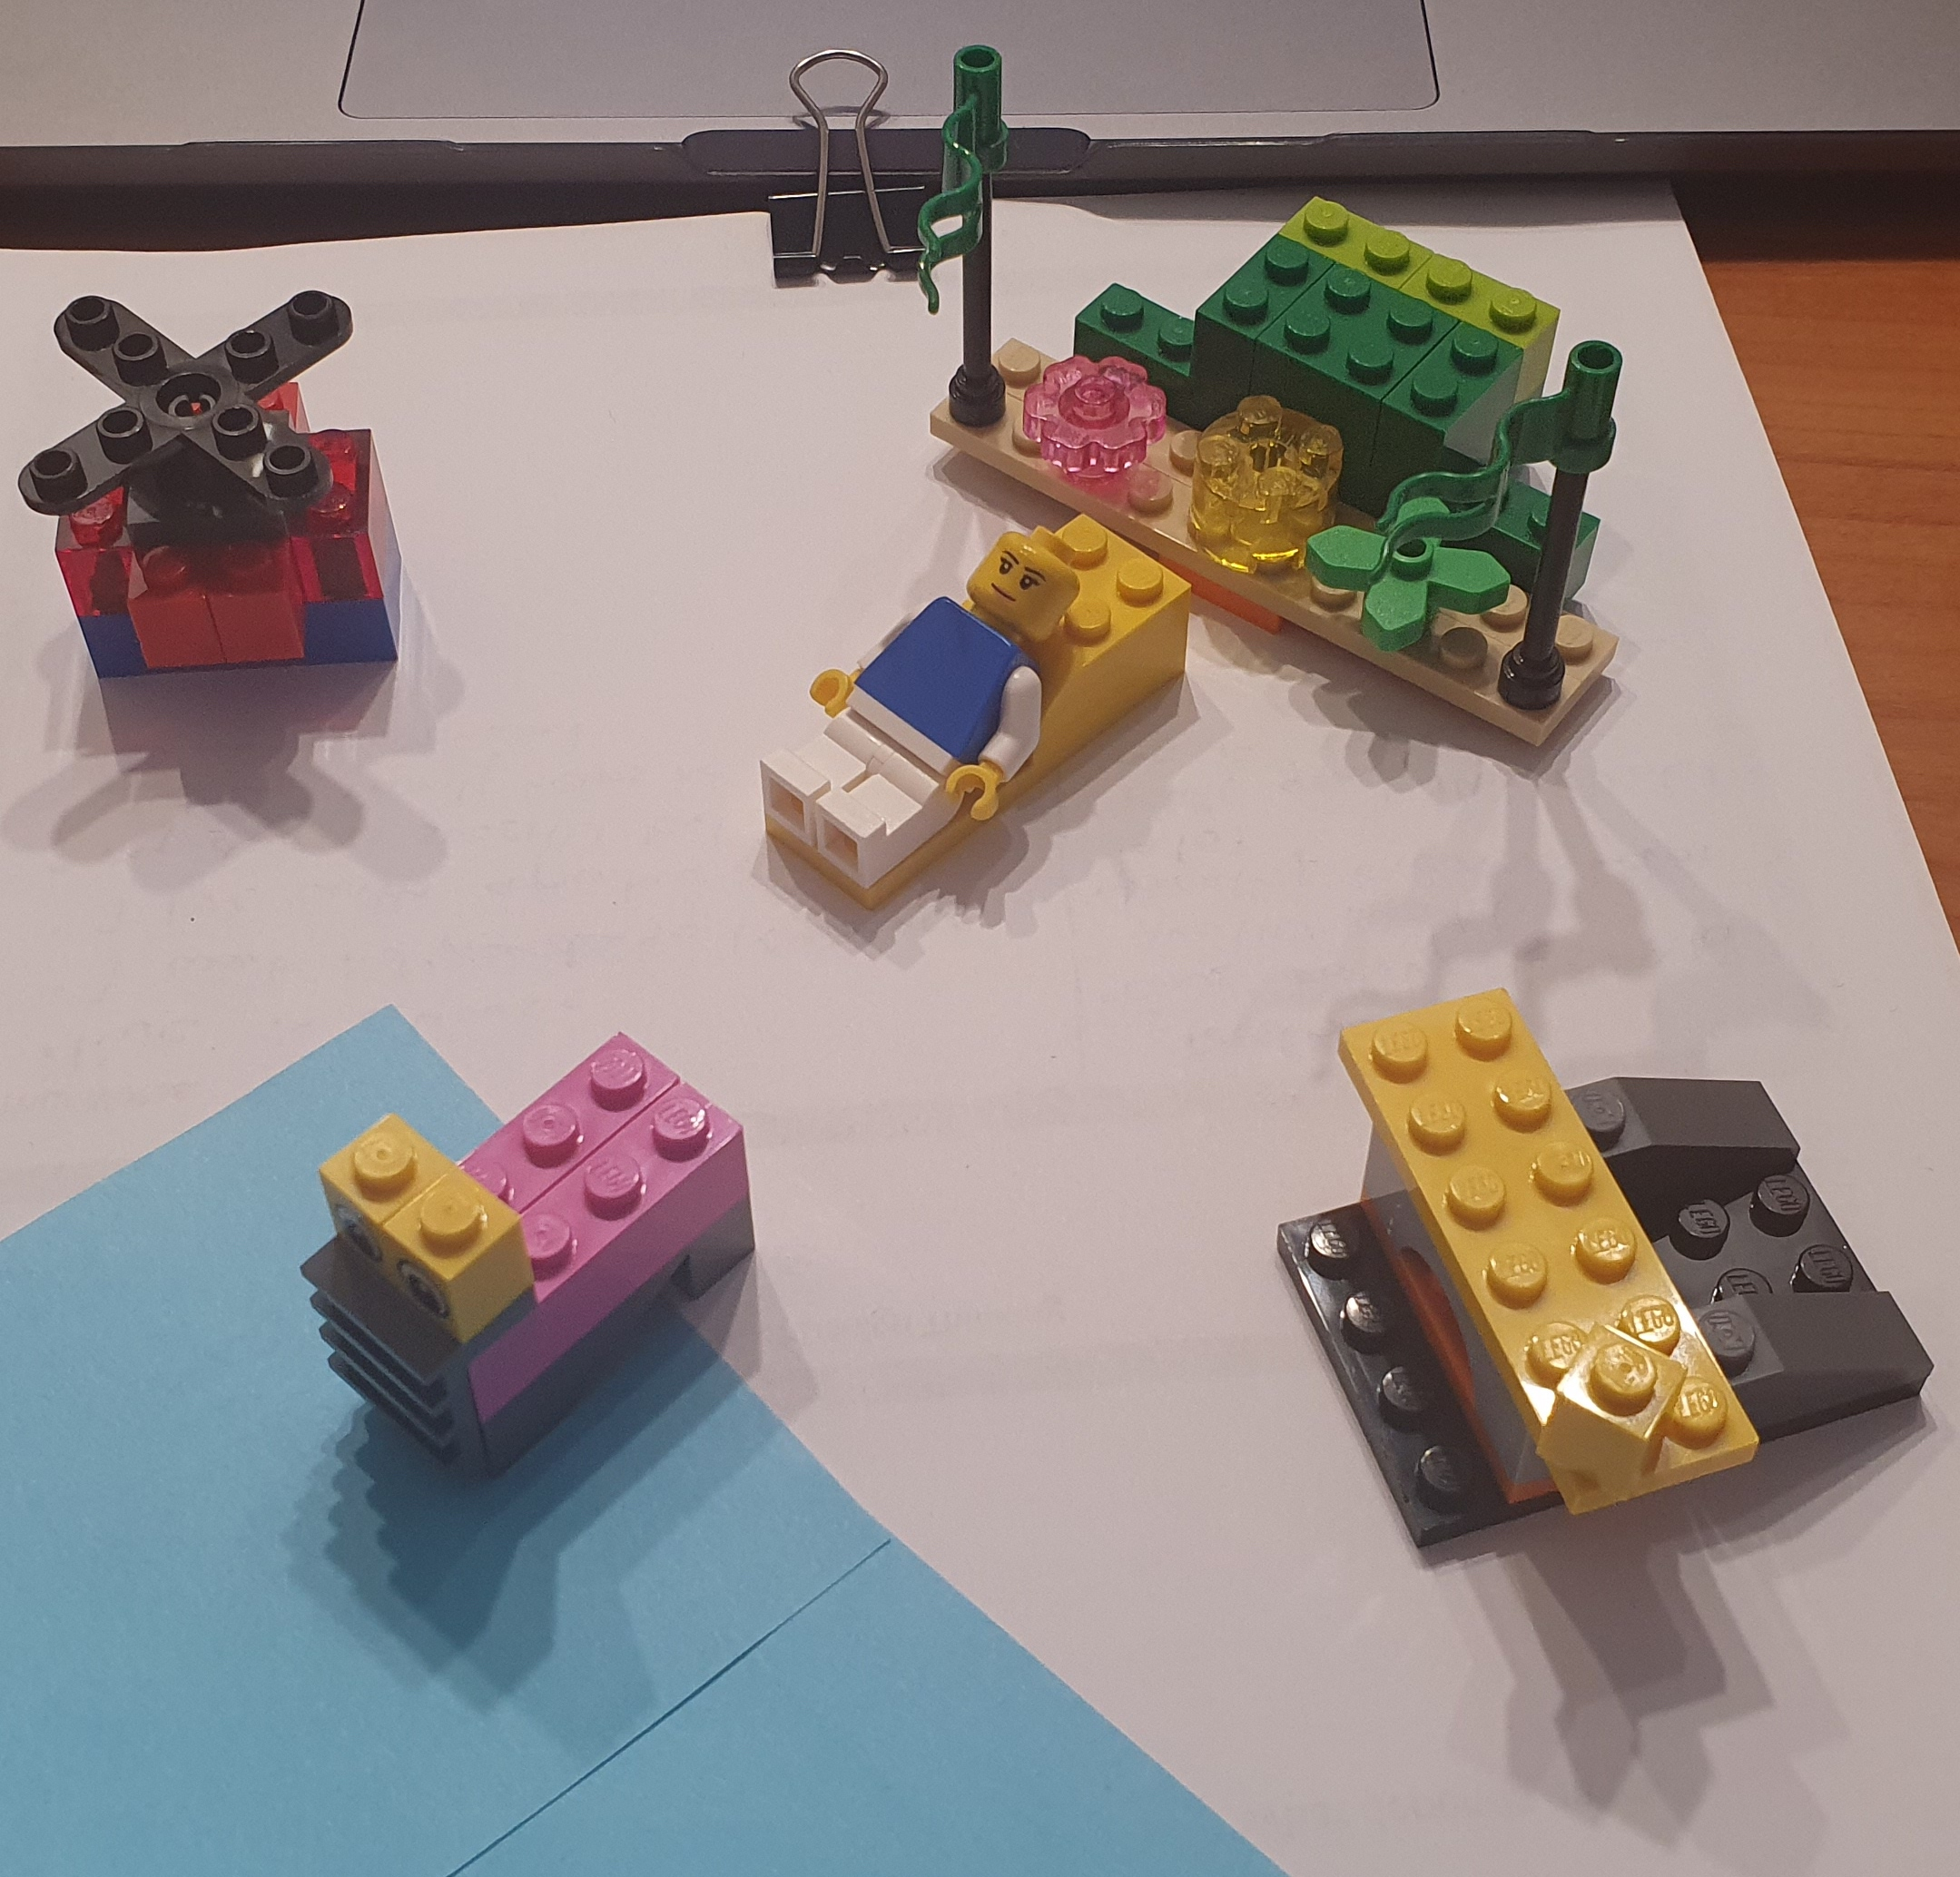
\includegraphics[width=7.7cm]{img/week_3_1.jpg}
        \end{center}
        \caption{``Working remote'' - Prototype of week 3}
        \label{fig:week3}
    \end{figure} 
    \begin{figure}[h]
        \begin{center}
            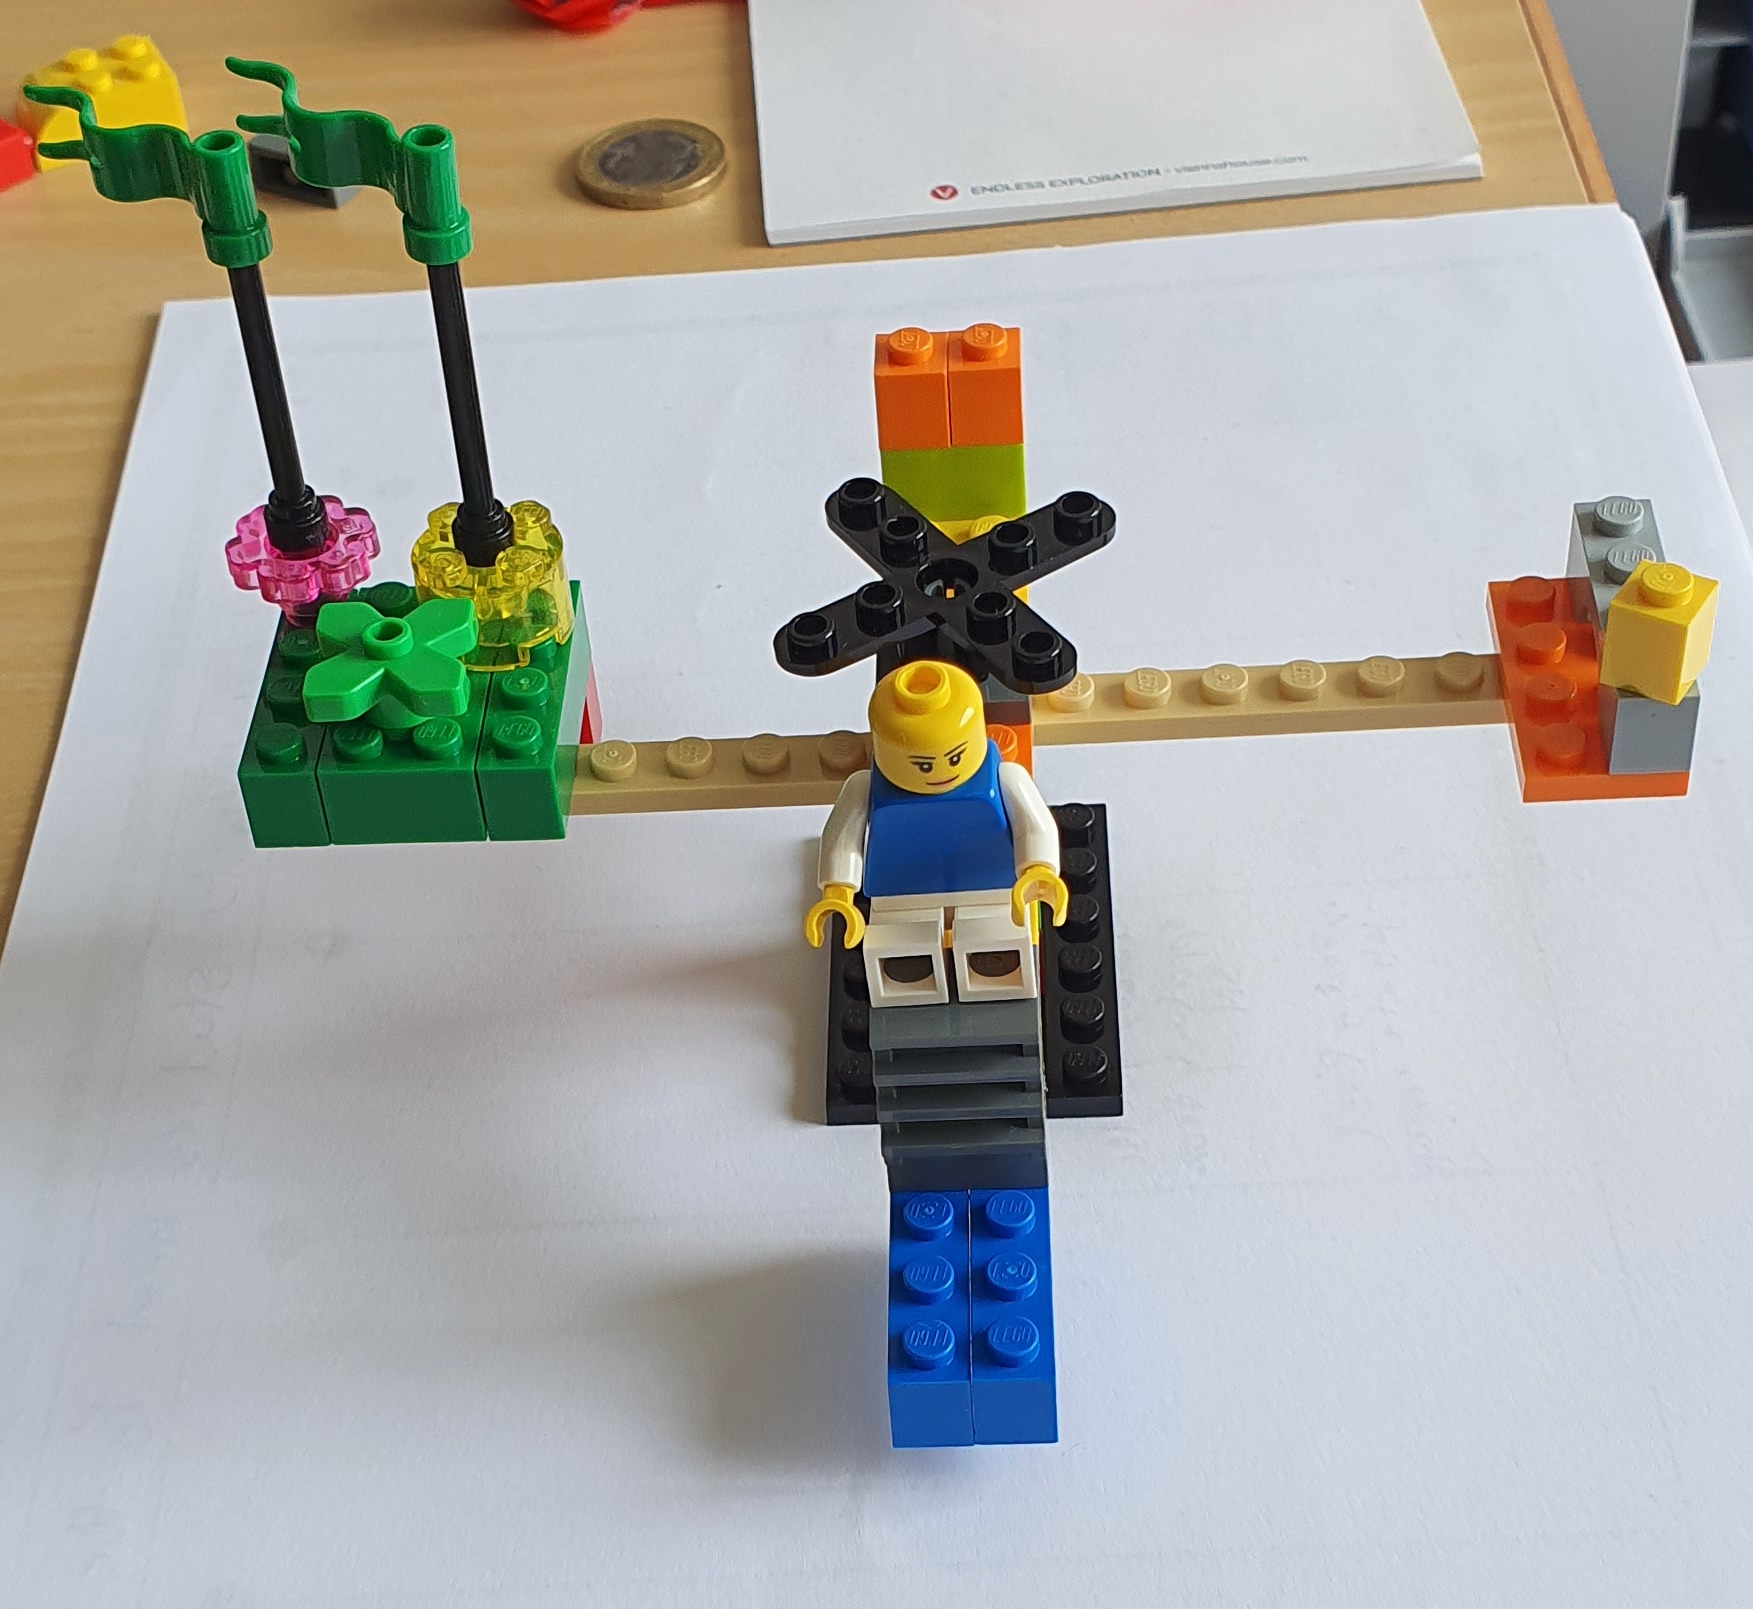
\includegraphics[width=7.7cm]{img/week_4.jpg}
        \end{center}
        \caption{``The game plan'' - Prototype of week 4}
        \label{fig:week4}
    \end{figure} 
\end{center}


\pagebreak
\subsection{Referenzen}
